\documentclass[12pt,compress,aspectratio=169]{beamer}
\usetheme{metropolis}
\setbeamersize{text margin left=.5cm,text margin right=.5cm}
\usepackage[lf]{carlito}
\usepackage{siunitx}
\usepackage{tikz}
\usepackage{mathpazo}
\usepackage{bm}
\usepackage{mathtools}
\usepackage[ISO]{diffcoeff}
\diffdef{}{ op-symbol=\mathsf{d} }
\usepackage{xcolor,colortbl}

\setmonofont{Ubuntu Mono}
\setlength{\parskip}{0pt}
\renewcommand{\baselinestretch}{1}

\sisetup{
  inter-unit-product=\cdot,
  per-mode=symbol
}

\tikzset{
  >=latex
}

%\newcommand{\iii}{\hat{\bm\imath}}
%\newcommand{\jjj}{\hat{\bm\jmath}}
%\newcommand{\kkk}{\hat{\bm k}}


\usetikzlibrary{patterns}

\title{Class 8: Rotational Motion of a Rigid Body, Part 2}
\subtitle{Advanced Placement Physics C}
\author[TML]{Dr.\ Timothy Leung}
\institute{Olympiads School}
\date{Updated: Summer 2022}

\newcommand{\pic}[2]{
  \includegraphics[width=#1\textwidth]{#2}
}
\newcommand{\eq}[2]{
  \vspace{#1}{\Large
    \begin{displaymath}
      #2
    \end{displaymath}
  }
}
%\newcommand{\iii}{\ensuremath\hat{\bm{\imath}}}
%\newcommand{\jjj}{\ensuremath\hat{\bm{\jmath}}}
%\newcommand{\kkk}{\ensuremath\hat{\bm{k}}}
\newcommand{\iii}{\ensuremath\hat\imath}
\newcommand{\jjj}{\ensuremath\hat\jmath}
\newcommand{\kkk}{\ensuremath\hat k}



\begin{document}

\begin{frame}
  \maketitle
\end{frame}



\section{Introduction}

\begin{frame}{Curvilinear vs. Rectilinear Motion}
  Kinematic quantities for rectilinear (translational) vs.\ curvilinear
  (circular) motion are related:

  \vspace{-.5in}{\Large
    \begin{align*}
      \vec r &\quad\rightarrow\quad \theta \\
      \vec v &\quad\rightarrow\quad \omega \\
      \vec a &\quad\rightarrow\quad \alpha
    \end{align*}
  }

  Dynamics:
  
  \vspace{-.5in}{\Large
    \begin{align*}
      m &\quad\rightarrow\quad I\\
      \vec F &\quad\rightarrow\quad \vec\tau\\
      \vec p=m\vec v &\quad\rightarrow\quad \vec L=I\omega
    \end{align*}
  }
\end{frame}



\begin{frame}{Laws of Motion}

  The laws of motion are also related between translational and rotational
  motion:
  
  \vspace{-.3in}{\Large
    \begin{align*}
      \vec F_\text{net}=\diff{\vec p}t &\quad\rightarrow\quad
      \vec\tau_\text{net}=\diff{\vec L}t \\
      \vec F_\text{net}=m \vec a &\quad\rightarrow\quad
      \vec\tau_\text{net}=I\vec\alpha
    \end{align*}
  }
\end{frame}



%\begin{frame}{Torque}
%  Recall the second law of motion for objects with constant mass:
%    
%  \eq{-.2in}{
%    \bm{F}_\text{net}=m\bm{a}
%  }
%
%  \vspace{-.1in}Is it also true for \emph{rotational} motion? If a net force
%  $\bm{F}_\text{net}$ causes the center of mass of an object to begin to
%  accelerate, what causes a mass to rotate?
%\end{frame}
%
%
%\section{Torque}
%
%\begin{frame}{Torque}
%  I have a rod on a table, and with my fingers, I push the two ends of the rod
%  with equal force $\textcolor{red!80!black}{F}$. \emph{What happens?}
%  \begin{center}
%    \begin{tikzpicture}[scale=1.5]
%      \fill[gray,draw=black,thick] (-2,-.1) rectangle (2,.1);
%      \begin{scope}[very thick, red!80!black,<-]
%        \draw(-1.8,-.1)--(-1.8,-.7) node[below]{$F$};
%        \draw( 1.8, .1)--( 1.8, .7) node[above]{$F$};
%      \end{scope}
%    \end{tikzpicture}
%  \end{center}
%  $\bm{F}_\text{net}=\bm{0}$, therefore $\bm{a}_{CM}=\bm{0}$. But it is also
%  obvious that the rod would \emph{rotate} instead.
%\end{frame}
%
%
%
%\begin{frame}{What is Torque?}
%  \textbf{Torque} (or \textbf{moment}) is the tendency for a force to change
%  the rotational motion of a body.
%  \begin{itemize}
%  \item A force $\bm{F}_a$ acting at a point some distance $\bm{r}$ (called the
%    \textbf{moment arm}) from a \textbf{fulcrum} (or \textbf{pivot}) at an angle
%    $\phi$ between $\bm{F}_a$ and $\bm{r}$
%  \item e.g.\ the force to twist a screw
%  \end{itemize}
%  In the example below, a force $\bm{F}$ is applied $\bm{r}$ away from
%  the pivot at an angle $\phi$. This generates a torque around the pivot.
%  \begin{center}
%    \begin{tikzpicture}[scale=2.8]
%      \begin{scope}[thick]
%        \draw[fill=gray!50](0,-.05) rectangle (2,.05);
%        \draw[fill=gray!50](0,0) circle (.15);
%      \end{scope}
%      \fill (0,0) circle (.03);
%      \begin{scope}[very thick]
%        \draw[red!70!black,->](0,0)--(1.8,0) node[midway,below]{$\bm{r}$};
%        \draw[blue!70!black,->](1.2,-.7)--(1.8,0) node[pos=0,below]{$\bm{F}$};
%        \draw[<->] (1.4,0) arc(180:229:.4)node[midway,left]{$\phi$};
%      \end{scope}
%    \end{tikzpicture}
%  \end{center}
%\end{frame}
%
%
%
%\begin{frame}{Torque}
%  Torque $\bm\tau$ is defined as the cross product of the force $\bm{F}$ and the
%  \textbf{moment arm} $\bm{r}$. The unit for torque is a \textbf{newton meter}
%  (\si{\newton\metre}).
%
%  \eq{-.25in}{
%    \boxed{\bm{\tau}=\bm{r}\times\bm{F}_a}
%  }
%
%  \vspace{-.1in}Its magnitude can be calculated in scalar form
%  using the angle $\phi$ between $\bm{F}$ and $\bm{r}$:
%
%  \eq{-.23in}{
%    \boxed{\tau=Fr\sin\phi}
%  }
%  \begin{center}
%    \begin{tabular}{l|c|c}
%      \rowcolor{pink}
%      \textbf{Quantity} & \textbf{Symbol} & \textbf{SI Unit} \\ \hline
%      Torque        & $\bm\tau$ & \si{\newton\metre} \\
%      Applied force & $\bm{F}_a$  & \si\newton \\
%      Moment arm (from fulcrum to force) & $\bm{r}$ & \si\metre \\
%      Angle between force and moment arm & $\phi$ & (no units)
%    \end{tabular}
%  \end{center}
%\end{frame}
%
%
%
%\begin{frame}{Example Problem}
%  \textbf{Example:} Find the net torque on point C.
%  \begin{center}
%    \begin{tikzpicture}[scale=2.65]
%      \fill[blue!40,draw=black,thick] (-1.65,-.12) rectangle (1.65,.12);
%      \draw[thick,<->](-1.5,-.25)--(1.5,-.25) node[midway,below]{\SI{3.}\metre};
%      \draw[thick,<->](-1.5,.25)--(0,.25) node[midway,above]{\SI{1.5}\metre};
%      \draw[dashed,thick](-2.2,0)--(2.2,0);
%      \draw[dashed,thick](0,0)--(0,.5);
%      \begin{scope}[orange,ultra thick,->]
%        \draw[rotate=-45](0,0)--(0,1.5)node[right]{\SI{30}\newton};
%        \draw[rotate around={30:(-1.5,0)}](-1.5,0)--(-2.5,0)
%        node[left]{\SI{20}\newton};
%        \draw[rotate around={-30:(1.5,0)}](1.5,0)--(2.2,0)
%        node[right]{\SI{10}\newton};
%      \end{scope}
%      \begin{scope}[thick,->]
%        \draw(0,.4)   arc(90:45:.4)  node[pos=.7,above]{\ang{45}};
%        \draw(-1.9,0) arc(180:210:.4)node[midway,left] {\ang{30}};
%        \draw(1.9,0)  arc(0:-30:.4)  node[midway,right]{\ang{30}};
%      \end{scope}
%      \fill (-1.5,0) circle(.1) node[white]{\textbf{A}};
%      \fill (   0,0) circle(.1) node[white]{\textbf{B}};
%      \fill ( 1.5,0) circle(.1) node[white]{\textbf{C}};
%    \end{tikzpicture}
%  \end{center}
%%  \uncover<2->{
%%    \textbf{Example 8b:} Now find the net torque on A.
%%  }
%\end{frame}
%
%
%
%
%
%%\begin{frame}{Torque}
%%  Going back to the example question:
%%  \begin{center}
%%    \begin{tikzpicture}
%%      \fill[black!75,draw=black!75] (-5,-.05) rectangle (5,.05);
%%      \fill (0,0) circle (.1);
%%      \draw[ultra thick](0,0)--(.5,-1.5)--(-.5,-1.5)--(0,0);
%%      \uncover<2->{
%%        \draw[ultra thick,red!75,->](0,0)--(-4.8,0) node[pos=.5,below]{$d_1$};
%%        \draw[ultra thick,red!75,->](-4.8,0)--(-4.8,-1)node[below]{$F_1$};
%%      }
%%      \uncover<3->{
%%        \draw[ultra thick,blue!60,->](0,0)--(4,0) node[pos=.5,below]{$d_2$};
%%        \draw[ultra thick,blue!60,->](4,0)--(4,-1.2) node[below]{$F_2$};
%%      }
%%    \end{tikzpicture}
%%  \end{center}
%%  \begin{itemize}
%%  \item<2->$F_1$ will rotate the board counter clockwise
%%  \item<3->$F_2$ will rotate the board clockwise
%%  \item<4->The beam will remain static (in equilibrium) if
%%
%%    \eq{-.2in}{ F_1d_1=F_2d_2 }
%%  \end{itemize}
%%\end{frame}
%
%
%
%\section{Angular Momentum}
%
%\begin{frame}{Angular Momentum}
%  Consider a mass $m$ connected to a massless beam rotates with velocity
%  $\bm{v}$ at a position $\bm{r}$ from the center (shown on the right). It has
%  an \textbf{angular momentum} ($\bm{L}$), defined as:
%  \begin{columns}
%    \column{.77\textwidth}
%    
%    \eq{-.32in}{
%      \boxed{\bm{L}=\bm{r}\times\bm{p}=m(\bm{r}\times\bm{v})}
%    }
%
%    \vspace{-.1in}Expanding the term with $\bm{v}=\bm\omega\times\bm{r}$, the
%    expression for angular momentum can now be expressed in quantities related
%    to rotations:
%
%    \eq{-.32in}{
%      \boxed{\bm{L}=m(\bm{r}\times\bm{v})
%        =m(\bm{r}\times(\bm\omega\times\bm{r}))
%        =mr^2\bm\omega}
%    }
%    
%    \vspace{-.2in}Or in scalar form:
%    
%    \eq{-.25in}{
%      \boxed{L=rmv=mr^2\omega}
%    }
%
%    \vspace{-.2in}The unit for angular momentum is a
%    \textbf{kilogram meter squared per second}
%    (\si{\newton\metre\squared\per\second}).
%    
%    \column{.23\textwidth}
%    \begin{tikzpicture}[scale=2.5]
%      \begin{scope}[rotate=70]
%        \fill[black!75,draw=black!75] (0,-.02) rectangle (2,.02);
%        \fill[blue!75,draw=blue,thick] (2,0) circle(.05);
%        \node(M) at (2,-.2) {$m$};
%        \fill (0,0) circle (.05);
%        \begin{scope}[very thick,->]
%          \draw[red!70!black](0,0)--(2,0)node[midway,right]{$\bm{r}$};
%          \draw (2,0)--(2,.5)node[left]{$\bm{v}$};
%        \end{scope}
%      \end{scope}
%    \end{tikzpicture}
%  \end{columns}
%\end{frame}
%
%
%
%\begin{frame}{Moment of Inertia}
%  Look again at the definition of angular momentum:
%    
%  \eq{-.2in}{
%    \bm{L}=\underbrace{mr^2}_{I}\bm\omega
%  }
%    
%  The quantity $I=mr^2$ is called the \textbf{moment of inertia} with a unit of
%  \textbf{kilogram meter squared} (\si{\kilo\gram\metre\squared}), and 
%
%  \eq{-.2in}{
%    \boxed{\bm{L}=I\bm\omega}
%  }
%
%  Momentum of inertia can be considered to be an object's ``rotational mass''
%
%\end{frame}
%
%
%
%\begin{frame}{Moment of Inertia}
%  For a \emph{single particle} of $m$ rotating at a distance $r$ from the pivot:
%  
%  \eq{-.2in}{
%    \boxed{I=mr^2}
%  }
%
%  For a \emph{collection of particles} rotating at $\omega$, each of mass
%  $m_i$ at distance $r_i$ from the pivot:
%
%  \eq{-.2in}{
%    \boxed{I=\sum m_ir_i^2}
%  }
%
%  For a \emph{continuous distribution of mass} about a pivot, integral calculus
%  is need to calculate the momentum of inertia:
%
%  \eq{-.25in}{
%    \boxed{I=\int r^2\dl m}
%  }
%\end{frame}
%
%
%
%\begin{frame}{Moment of Inertia}
%  \centering
%  \pic{.7}{mic}
%\end{frame}
%
%
%
%\begin{frame}{Angular Momentum and Moment of Inertia}
%  Linear and angular momentum have very similar expressions
%    
%  \vspace{-.4in}{\Large
%    \begin{align*}
%      \bm{p}&=m\bm{v}\\
%      \bm{L}&=I\bm\omega
%    \end{align*}
%  }
%  
%  \vspace{-.25in}Just as $\bm{p}$ describes the overall \emph{translational}
%  state of motion of a physical system, $\bm{L}$ describes its overall
%  \emph{rotational} state
%\end{frame}
%
%
%
%\section{Laws of Motion}
%
%\begin{frame}{Equilibrium: First Law of Motion}
%  An object is in \textbf{translational equilibrium} is when the net force
%  acting on it is zero:
%  
%  \eq{-.2in}{
%    \bm{F}_\text{net}=\bm{0}
%  }
%
%  This does \emph{not} mean that the object has no translational motion; it
%  just means that the object's overall \emph{transtational state} is not
%  changing, i.e.\ linear momentum $\bm{p}$ is constant. For
%  constant mass $m$, this means that $\bm{a}=\bm{0}$.
%\end{frame}
%
%
%
%
%\begin{frame}{Equilibrium: First Law of Motion}
%  Likewise, an object is in \textbf{rotational equilibrium} when the net torque
%  acting on it is zero:
%
%  \eq{-.2in}{
%    \bm{\tau}_\text{net}=\bm{0}
%  }
%  
%  This does \emph{not} mean that the object has no rotational motion; it just
%  means that the object's overall \emph{rotational state} is not changing,
%  i.e.\  angular momentum $\bm{L}$ is constant. For constant moment of inertia
%  $I$, this means that $\bm\alpha=\bm{0}$.
%\end{frame}
%
%
%
%\begin{frame}{Second Law of Motion for Rotational Motion}
%  The net torque is the time rate of change of angular momentum:
%
%  \eq{-.2in}{
%    \bm{\tau}_\text{net}=\bm{r}\times\bm{F}_\text{net}
%    =\bm{r}\times\diff{\bm{p}}t
%    =\diff{(\bm{r}\times\bm{p})}t\;\;\longrightarrow\;\;
%    \boxed{\bm{\tau}_\text{net}=\diff{\bm{L}}t}
%  }
%  \begin{itemize}
%  \item If the net torque on a system is zero, then the rate of change
%    of angular momentum is zero, and we say that the angular momentum is
%    conserved. 
%  \item e.g.\ When an ice skater starts to spin and draws his arms inward.
%    Since angular momentum is conserved, a decrease in $r$ means an
%    increase in $\omega$.
%  \end{itemize}
%\end{frame}
%
%
%
%\begin{frame}{Second Law of Motion for Translational Motion}
%  For translational motion, the general form of the first and second laws of
%  motion states that the net force is rate of change of the object's momentum:
%
%  \eq{-.2in}{
%    \bm{F}_\text{net}=\diff{\bm{p}}t
%  }
%
%  For objects with constant mass, this reduces to the more familiar form:
%
%  \eq{-.2in}{
%    \bm{F}=m\bm{a}
%  }
%\end{frame}
%
%
%
%\begin{frame}{Second Law of Motion for Rotational Motion}
%  Likewise, the second law of motion for rotational motion has a similar
%  form, but with torque $\bm\tau$ replacing force $\bm{F}$, and angular
%  momentum $\bm{L}$ replacing linear momentum $\bm{p}$:
%
%  \eq{-.2in}{
%    \boxed{
%      \bm{\tau}_\text{net}=\diff{\bm{L}}{t}
%    }
%  }
%
%  For objects with constant momentum of inertia $I$, this reduces to:
%
%  \eq{-.2in}{
%    \bm\tau_\text{net}=I\bm\alpha
%  }
%\end{frame}
%
%
%
%\begin{frame}{But there is no rotational motion, is there?}
%  Even when there is no apparent rotational motion, it does not necessarily
%  mean that angular momentum is zero! In this case, mass $m$ travels along a
%  straight path at constant velocity (uniform motion), but the angular momentum
%  around point $P$ is not zero:
%  \begin{center}
%    \begin{tikzpicture}
%      \draw[dashed](-5,0)--(5,0);
%      \draw[very thick,red!70!black,->](-5,0)--(-3,0) node[below]{$\bm{v}$};
%      \tikzstyle{balloon}=[ball color=red!70!black];
%      \shade[balloon] (-5,0) circle(.2) node[above left,red!70!black]{$m$};
%      \fill (0,-2) circle(.05) node[below]{$P$};
%      \draw[very thick,blue!70!black,->](0,-2)--(-5,0)
%      node[midway,below left]{$\bm{r}$};
%      \uncover<2->{
%        \draw[dotted](0,0) circle(.2) node[above left]{$m$};
%        \draw[thick,red!50,->](.2,0)--(2,0)node[right]{$\bm{v}$};
%        \draw[thick,blue!50,->](0,-2)--(0,0) node[midway,left]{$\bm{r}$};
%      }
%      \uncover<3->{
%        \draw[dotted](4,0) circle(.2) node[above left]{$m$};
%        \draw[thick,red!50,->](4.2,0)--(6,0)node[right]{$\bm{v}$};
%        \draw[thick,blue!50,->](0,-2)--(4,0)node[midway,above left]{$\bm{r}$};
%      }
%    \end{tikzpicture}
%  \end{center}
%  \uncover<4>{
%    Since there is no force and no torque acting on the object, both the linear
%    momentum ($\bm{p}=m\bm{v}$) and angular momentum
%    ($\bm{L}=\bm{r}\times\bm{v}$) are constant.
%  }
%\end{frame}
%
%
%
%\begin{frame}{Example Problem}
%  \textbf{Example:} A skater extends her arms (both arms!), holding a
%  \SI{2.}{\kilo\gram} mass in each hand. She is rotating about a vertical axis
%  at a given rate. She brings her arms inward toward her body in such a way that
%  the distance of each mass from the axis changes from \SI{1.}\metre to
%  \SI{.50}\metre. Her rate of rotation (neglecting her own mass) will?
%\end{frame}
%
%
%
%
%\begin{frame}{Example Problem}
%  \textbf{Example:} A \SI{1.}{\kilo\gram} mass swings in a vertical circle
%  after having been released from a horizontal position with zero initial
%  velocity. The mass is attached to a massless rigid rod of length
%  \SI{1.5}\metre. What is the angular momentum of the mass, when it is in its
%  lowest position?
%\end{frame}



\begin{frame}{Solving Rotational Problems}
  When solving for rotational problems like the ones described in the previous
  sections:
  \begin{itemize}
  \item Draw a free-body diagram to account for all forces
  \item The direction of friction force is not always obvious
  \item The magnitude of any static friction force cannot be assumed to be at
    maximum.
  \item If the object is to change its rotational state, there must be a net
    torque causing it.
  \end{itemize}
\end{frame}



\begin{frame}{Solving Rotational Problems}
  Once the free-body diagram is complete, the forces should break down into
  their \emph{forces} into $\iii$, $\jjj$ and $\kkk$ components. If the axes
  are defined properly, only one direction should have acceleration (usually
  $\iii$), i.e.:
  
  \eq{-.2in}{
    \sum F_x=ma \quad\quad \sum F_y=0 \quad\quad \sum F_z=0
  }

  There are also three equations for rotation, and torque is only applied in one
  direction (likely $\kkk$):
    
  \eq{-.2in}{
    \sum\tau_x=0 \quad\quad \sum\tau_y=0 \quad\quad \sum\tau_z=I_z\alpha
  }
\end{frame}



\begin{frame}{Solving Rotational Problems}
  For rotational motion dynamics equation:
  \begin{enumerate}
  \item Relate the force(s) that causes rotational motion to the net torque

    \eq{-.2in}{
      \tau_\text{net}=\sum_i F_ir_i
    }
  \item Substitute the expression for momentum of inertia (which has both mass
    and radius terms in it) into the equation for rotational motion
  \item Relate angular acceleration to linear acceleration, if applicable:

    \eq{-.25in}{
      \alpha=\frac{a}R
    }
  \end{enumerate}
  Now there are two equations with force and acceleration terms.
\end{frame}


\begin{frame}{Problems with Only Rotations}


\end{frame}



\section{Pure Rolling Problems}

\begin{frame}{Pure Rolling Problems}
  A smooth solid sphere of constant density rolls along a smooth surface
  without slipping (called \textbf{pure rolling}). We assume that:
  \begin{itemize}
    \item Both the sphere and the surface are both perfectly rigid (they
      do not deform)
    \item The sphere and the surface are both perfectly smooth without defects
      even at the microscopic level
  \end{itemize}
  The free-body diagram: %in Figure \ref{roll-flat}. Notice that
%\emph{there is no friction between the sphere and the surface}. Since there is
%neither a net force nor a net torque acting on the sphere, the translational
%and rotational states are constant in time. In theory (if our assumptions are
%correct), the sphere with translational velocity $\bm{v}$ and angular velocity
%$\bm\omega$ (where $\bm{v}=\bm{\omega}\times R$) will roll along forever.
  \begin{center}
    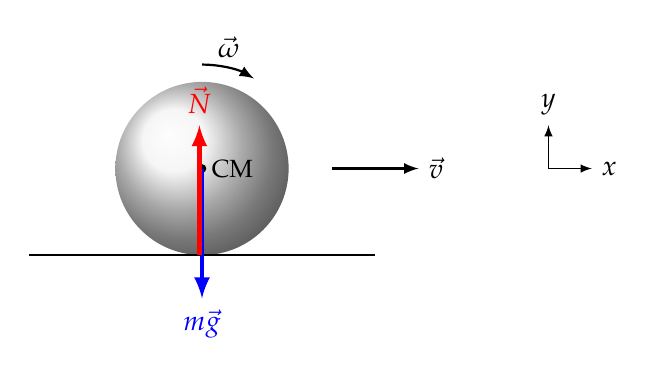
\begin{tikzpicture}[scale=1.1]
      \shade[ball color=gray!10](0,0) circle(1);
      \draw[thick](-2,-1)--(2,-1);
      \draw[thick,->](1.5,0)--(2.5,0) node[right]{$\vec v$};
      \draw[thick,->](0,1.2) arc(90:60:1.2) node[midway,above]{$\vec\omega$};
      \draw[->](4,0)--(4.5,0) node[right]{$x$};
      \draw[->](4,0)--(4,.5) node[above]{$y$};
      \fill(0,0) circle(.05) node[right]{\small CM};
      \begin{scope}[->,ultra thick]
        \draw[blue](0,0)--(0,-1.5) node[below]{$m\vec g$};
        \draw[red](-.03,-1)--(-.03,.5) node[above]{$\vec N$};
      \end{scope}
    \end{tikzpicture}
  \end{center}
\end{frame}



\begin{frame}{Pure Rolling Problems}
  The free-body diagram is simple enough that we can see that:
  \begin{columns}
    \column{.65\textwidth}
    \begin{itemize}
    \item There is no friction
    \item Neither gravity ($m\vec g$) nor normal force ($\vec N$) generate a
      torque about the CM
    \item $\sum F=0$ and $\sum\tau=0$, therefore
    \item The translational state ($\vec v$) and rotational state ($\omega$) are
      constant in time
    \item In \emph{theory}, this sphere will roll along with velocity $\vec v$
      and angular velocity $\omega=v/R$ forever
    \end{itemize}

    \column{.35\textwidth}
    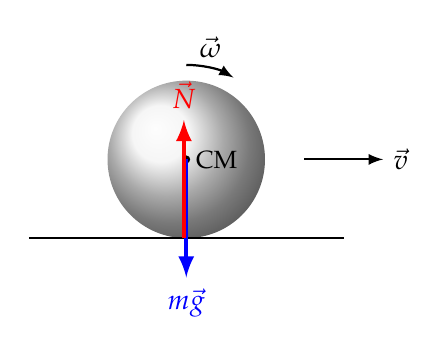
\begin{tikzpicture}
      \shade[ball color=gray!10](0,0) circle(1);
      \draw[thick](-2,-1)--(2,-1);
      \draw[thick,->](1.5,0)--(2.5,0) node[right]{$\vec v$};
      \draw[thick,->](0,1.2) arc(90:60:1.2) node[midway,above]{$\vec\omega$};
      \fill(0,0) circle(.05) node[right]{\small CM};
      \begin{scope}[->,ultra thick]
        \draw[blue](0,0)--(0,-1.5) node[below]{$m\vec g$};
        \draw[red](-.03,-1)--(-.03,.5) node[above]{$\vec N$};
      \end{scope}
    \end{tikzpicture}
  \end{columns}
\end{frame}


\begin{frame}{Reality: Rolling Resistance}
  In reality, the rolling ball will slow down and eventually come to a stop,
  because \emph{nothing is perfectly rigid}: both the ball and the surface
  deform when they make contact
  \begin{columns}
    \column{.65\textwidth}
    \begin{itemize}
      %\begin{itemize}
      %\item e.g.\ a tire flattens when it makes contact with the ground
      %\end{itemize}
    \item The normal force is larger in magnitude on the front side than on the
      other
    \item $N$ exerts both a horizontal force to slow down the ball, as well as a
      torque to slow down its rotation
    \item The normal force does not point toward the CM because of the
      deformation.
    \end{itemize}

    \column{.35\textwidth}
    \vspace{.3in}
    \pic1{OAGZy}
  \end{columns}
\end{frame}




\begin{frame}{Rolling with Slipping}
\end{frame}




\begin{frame}{Rolling on an Inclined Surface}
  For a rigid and smooth sphere of radius $R$ rolling down a ramp of angle
  $\phi$ without slippage down a ramp of angle $\theta$.

  \vspace{.2in}
  \begin{columns}
    \column{.35\textwidth}
    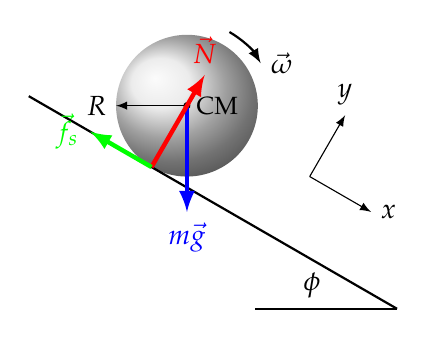
\begin{tikzpicture}[scale=.9]
      \begin{scope}[rotate=-30]
        \shade[ball color=gray!20](0,0) circle(1);
        \draw[thick](-2,-1)--(4,-1);
        \draw[->,rotate=30](0,0)--(-1,0) node[left]{$R$};
        \draw[thick,->](0,1.2) arc(90:60:1.2) node[right]{$\vec\omega$};
        \draw[->](2,0)--(3,0) node[right]{$x$};
        \draw[->](2,0)--(2,1) node[above]{$y$};
        \fill(0,0) circle(.05) node[right]{\small CM};
        \begin{scope}[->,ultra thick]
          \draw[blue,rotate=30](0,0)--(0,-1.5) node[below]{$m\vec g$};
          \draw[red](0,-1)--(0,.5) node[above]{$\vec N$};
          \draw[green](.0,-1)--(-1,-1) node[left]{$\vec f_s$};
        \end{scope}
        \begin{scope}[rotate around={30:(4,-1)}]
          \draw[thick](4,-1)--(2,-1) node[pos=.6,above]{$\phi$};
        \end{scope}
      \end{scope}
    \end{tikzpicture}
%  \caption{Force diagram on a smooth solid sphere of radius $R$ rolling down a
%    smooth ramp without slipping. The ball travels distance $d$ to the bottom
%    of the ramp.}
    %  \label{roll-ramp}

    \column{.65\textwidth}
    Three forces act on the sphere as it rolls down the ramp
    \begin{itemize}
    \item The weight ($mg$) of the sphere acts at the CM
    \item The normal force ($N$) acts at the point of contact
    \item The static friction ($f_s$) act at the point of contact
    \end{itemize}
    Only static friction generates a torque about the CM in the clockwise
    direction
    \begin{itemize}
    \item If $f_s$ is not present, there would have been nothing that causes
      the sphere to rotate.
    \end{itemize}
  \end{columns}
\end{frame}



\begin{frame}{Rolling on an Inclined Surface}
  \begin{columns}
    \column{.33\textwidth}
    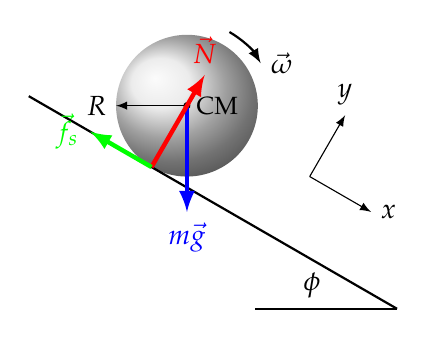
\begin{tikzpicture}[scale=.9]
      \begin{scope}[rotate=-30]
        \shade[ball color=gray!20](0,0) circle(1);
        \draw[thick](-2,-1)--(4,-1);
        \draw[->,rotate=30](0,0)--(-1,0) node[left]{$R$};
        \draw[thick,->](0,1.2) arc(90:60:1.2) node[right]{$\vec\omega$};
        \draw[->](2,0)--(3,0) node[right]{$x$};
        \draw[->](2,0)--(2,1) node[above]{$y$};
        \fill(0,0) circle(.05) node[right]{\small CM};
        \begin{scope}[->,ultra thick]
          \draw[blue,rotate=30](0,0)--(0,-1.5) node[below]{$m\vec g$};
          \draw[red](0,-1)--(0,.5) node[above]{$\vec N$};
          \draw[green](.0,-1)--(-1,-1) node[left]{$\vec f_s$};
        \end{scope}
        \begin{scope}[rotate around={30:(4,-1)}]
          \draw[thick](4,-1)--(2,-1) node[pos=.6,above]{$\phi$};
        \end{scope}
      \end{scope}
    \end{tikzpicture}
%  \caption{Force diagram on a smooth solid sphere of radius $R$ rolling down a
%    smooth ramp without slipping. The ball travels distance $d$ to the bottom
%    of the ramp.}
    %  \label{roll-ramp}

    \column{.67\textwidth}
    To solve this problem, there are three dynamics equations:
  %axes\footnote{the $\kkk$ axis points \emph{out} of the page. Counter-clockwise
    %  rotational motion is positive, while clockwise rotational motion is negative}

    \vspace{-.4in}{\Large
      \begin{align*}
        \sum F_x&=mg\sin\theta-f_s=ma\\
        \sum F_y&=N-mg\cos\theta=0\\
        \sum\tau &=Rf_s=I\alpha
      \end{align*}
    }
    
    %\textbf{Don't be so sure about what $\mu_s$ tells us.}
    \vspace{-.2in}At this point, static friction $f_s$ is \emph{not} known.
    The coefficient of static friction ($\mu_s$) only tells us the
    \emph{maximum} static friction, not the \emph{actual} friction. (We will
    instead use it to check if the answer makes sense.)
  \end{columns}
\end{frame}



\begin{frame}{Rolling on an Inclined Surface}
  \begin{columns}
    \column{.33\textwidth}
    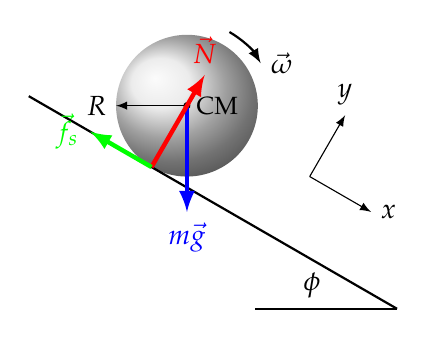
\begin{tikzpicture}[scale=.9]
      \begin{scope}[rotate=-30]
        \shade[ball color=gray!20](0,0) circle(1);
        \draw[thick](-2,-1)--(4,-1);
        \draw[->,rotate=30](0,0)--(-1,0) node[left]{$R$};
        \draw[thick,->](0,1.2) arc(90:60:1.2) node[right]{$\vec\omega$};
        \draw[->](2,0)--(3,0) node[right]{$x$};
        \draw[->](2,0)--(2,1) node[above]{$y$};
        \fill(0,0) circle(.05) node[right]{\small CM};
        \begin{scope}[->,ultra thick]
          \draw[blue,rotate=30](0,0)--(0,-1.5) node[below]{$m\vec g$};
          \draw[red](0,-1)--(0,.5) node[above]{$\vec N$};
          \draw[green](.0,-1)--(-1,-1) node[left]{$\vec f_s$};
        \end{scope}
        \begin{scope}[rotate around={30:(4,-1)}]
          \draw[thick](4,-1)--(2,-1) node[pos=.6,above]{$\phi$};
        \end{scope}
      \end{scope}
    \end{tikzpicture}

    \column{.67\textwidth}
    For non-slip case, angular and translational acceleration are related using
    relative motion:

    \eq{-.3in}{ a=\alpha R}
    
    \vspace{-.22in}Solving for the static friction:

    \eq{-.15in}{
      f_s=\frac{I\alpha}R=
      \frac25mR^2\cdotp\frac aR\cdotp\frac1R=\frac25ma
    }

    It is substituted into the force equation in the $\iii$ direction to
    solve for the acceleration of the CM down the ramp:

    \eq{-.2in}{
        mg\sin\theta-\frac25 ma =ma%\rightarrow
    }
  \end{columns}
\end{frame}


\begin{frame}{Rolling on an Inclined Surface}
  \begin{columns}
    \column{.33\textwidth}
    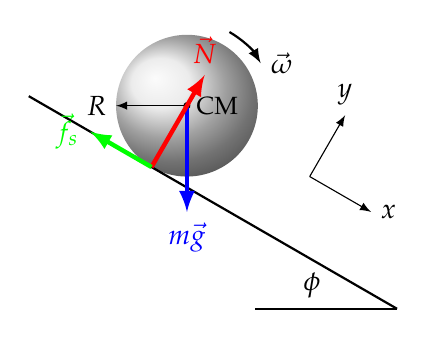
\begin{tikzpicture}[scale=.9]
      \begin{scope}[rotate=-30]
        \shade[ball color=gray!20](0,0) circle(1);
        \draw[thick](-2,-1)--(4,-1);
        \draw[->,rotate=30](0,0)--(-1,0) node[left]{$R$};
        \draw[thick,->](0,1.2) arc(90:60:1.2) node[right]{$\vec\omega$};
        \draw[->](2,0)--(3,0) node[right]{$x$};
        \draw[->](2,0)--(2,1) node[above]{$y$};
        \fill(0,0) circle(.05) node[right]{\small CM};
        \begin{scope}[->,ultra thick]
          \draw[blue,rotate=30](0,0)--(0,-1.5) node[below]{$m\vec g$};
          \draw[red](0,-1)--(0,.5) node[above]{$\vec N$};
          \draw[green](.0,-1)--(-1,-1) node[left]{$\vec f_s$};
        \end{scope}
        \begin{scope}[rotate around={30:(4,-1)}]
          \draw[thick](4,-1)--(2,-1) node[pos=.6,above]{$\phi$};
        \end{scope}
      \end{scope}
    \end{tikzpicture}

    \column{.67\textwidth}
    The acceleration of the center of mass is therefore:

    \eq{-,2in}{
      a=\frac57 g\sin\theta
    }

    \vspace{-.1in}Compare this to an object \emph{sliding} without friction
    down the same ramp, which is higher than the pure rolling case.
    
    \eq{-.25in}{
      a=g\sin\theta
    }
    
%The simplest explanation is that some of the gravitational potential energy is
%converted to both translational and rotational kinetic energies, while for the
%sliding case, all of the potential energy is converted into translational
%kinetic energy.
%If this is indeed the case, it means that the sphere will actually slip while
%rolling down the ramp, and the friction at the contact point is in fact kinetic
%friction.

    \vspace{-.2in}If the sphere starts from rest, the speed of the sphere when
    it reaches the bottom of the ramp, a distance $d$ away, would be:

    \eq{-.2in}{
      v=\sqrt{2ad}=\sqrt{\frac{10}7gd\sin\theta}
    }

%There is, of course, one ``sanity check'' that must be done, that is to make
%sure that the friction calculated in Eq.~\ref{f_s} has not exceeded the maximum
%static friction, given by
%\begin{equation}
%  f_s\leq\mu_s N
%  \label{maxf}
%\end{equation}
%Combining the expression for $f_s$ in Eq.~\ref{f_s}, the acceleration in
%Eq.~\ref{pure-roll-accel}, and the normal force on an incline, Eq.~\ref{maxf}
%becomes:
%\begin{align}
%  f_s&\leq\mu_sN\\
%  \frac27mg\sin\theta&\leq\mu_smg\cos\theta\\
%  \frac27\tan\theta&\leq\mu_s
%\end{align}
%If the ramp angle is too steep, then the friction will transition from static
    %to kinetic, which is a much more difficult problem.

  \end{columns}
\end{frame}



\section{Work \& Energy in Rotational Motion}

\begin{frame}{Mechanical Work}
  For translational motion, mechanical work is defined as

  \eq{-.2in}{
    W_t=\int_{x_1}^{x_2}\vec F\cdot\dl\vec x
  }

  For rotational motion, mechanical work is defined similarly as:

  \eq{-.2in}{
    \boxed{
      W_r=\int_{\theta_1}^{\theta_2}\tau\cdot\dl\theta
    }
  }

  The work-energy theorem still applies to rotational motion, i.e.;

  \eq{-.25in}{
    W_r=\Delta K_r
  }
\end{frame}



\begin{frame}{Rotational Kinetic Energy}
  To find the kinetic energy of a rotating system of particles (discrete number
  of particles, or continuous mass distribution), we sum the
  kinetic energies of the individual particles:
    
  \eq{-.1in}{
    K_r=\sum_i\frac12m_iv_i^2=\sum\frac12m_i(r_i\omega)^2
    =\frac12\left(\sum_i m_ir_i^2\right)\omega^2
  }
  
  It's no surprise that rotational kinetic energy is given by:
  
  \eq{-.2in}{
    \boxed{K_r=\frac12I\omega^2}
  }
\end{frame}



\begin{frame}{Kinetic Energy of a Rotating System}
  The total kinetic energy of a rotating system is the sum of its translational
  and rotational kinetic energies at its center of mass:

  \eq{-.2in}{
    \boxed{K=K_t+K_r=\frac12mv_\text{CM}^2+\frac12I_\text{CM}\omega^2}
  }
  
  In this case, $I_\text{CM}$ is calculated at the center of
  mass. For simple problems, we only need to compute rotational kinetic energy
  at the pivot:

  \eq{-.2in}{
    \boxed{K=\frac12I_\text{P}\omega^2}
  }
  
  In this case, the $I_\text{P}$ is calculated at the pivot.
  \textbf{IMPORTANT:} $I_\text{CM}\neq I_\text{P}$
\end{frame}



\begin{frame}{Parallel Axis Theorem}
  \begin{columns}
    \column{.35\textwidth}
    \pic{1}{Steiner}
    
    \column{.65\textwidth}
    The \textbf{parallel axis theorem} relates the moment of inertia of an
    object along two different but parallel axis by:

    \eq{-.2in}{
      \boxed{I=I_\text{CM}+md^2}
    }
  \end{columns}
\end{frame}
\end{document}
